\chapter{Bezpieczeństwo systemów komputerowych}

Materiały teoretyczne zostały opracowane na podstawie \href{https://moodle.mimuw.edu.pl/course/view.php?id=1490}{slajdów Tomasza Kazany}.

\textbf{Kod do Moodle:} BSK2022.8b52-g8

\subsection{Podstawa programowa}
\begin{enumerate}
    \item Podstawy \textbf{kryptografii}.
    \item Infrastruktura \textbf{klucza publicznego}.
    \item \textbf{Modele i klasy bezpieczeństwa} systemów informatycznych.
    \item \textbf{Modele uwierzytelniania}, strategie kontroli dostępu.
    \item \textbf{Bezpieczeństwo protokołów komunikacyjnych} i aplikacji.
    \item Praktyczna \textbf{ochrona systemów operacyjnych} i usług aplikacyjnych z wykorzystaniem izolacji, ścian ogniowych, VPN, TLS, PGP.
    \item Problematyka \textbf{bezpiecznego programowania}.
    \item Zagrożenia związane z \textbf{przestępczością elektroniczną}.
\end{enumerate}

\section{Klucz symetryczny}

\subsection{Historyczne szyfrowanie z kluczem symetrycznym}

\textbf{Szyfr Cezara}:

np. A -> E, B-> F, ... - przesuwamy alfabet np. o 4

Ogólniej \textbf{szyfr zastępowy (permutacyjny)}

np. E -> W, S -> E, A -> D, ...

ESSA -> WEED

Wszystkie te szyfry działają o wcześniej potajemnie ustalony \textbf{tajny klucz (klucz prywatny)}.

Enigma - maszyna szyfrująca używana przez Niemców podczas WWII też tak działała.

\begin{figure}[H]
    \centering
    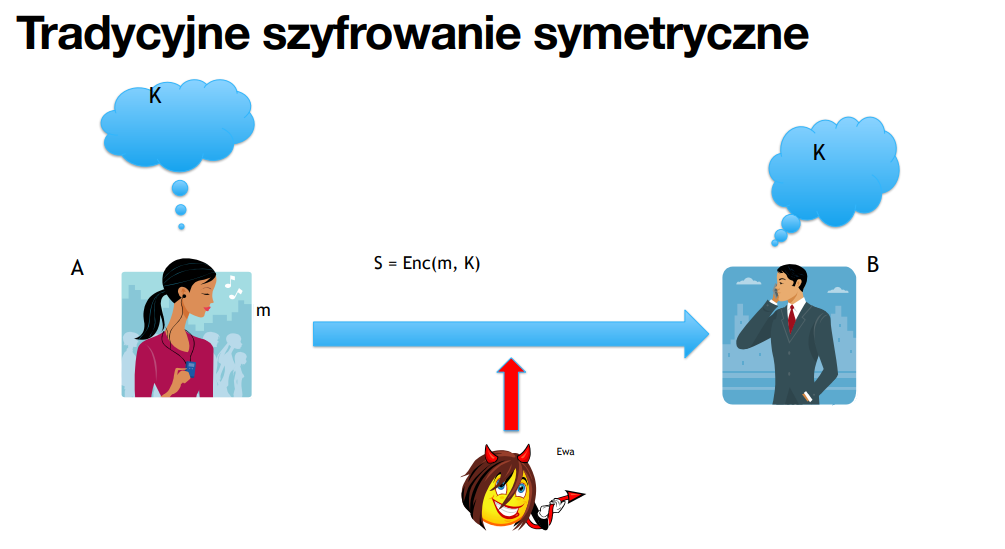
\includegraphics[width=0.75\textwidth]{rozdziały/images/BSK/tradycyjne-szyfrowanie-symetryczne.png}
\end{figure}

Formalnie:

m - wiadomość

K - klucz symetryczny

S - szyfrogram

Szyfrowanie: S = Enc(m,K)

Deszyfrowanie: Dec(S,K)

Poprawność: Dec((Enc(m,K),K)=m

Nawet jak Ewa zna szyfrogram, funkcje Dec i Enc to bez K nie jest w stanie rozszyfrować wiadomości.

Poprawna definicja bezpieczeństwa to, że na podstawie S przeciwnik nie pozna żadnej dodatkowej informacji o m - formalnie: rozkład m i Enc(m, K) są niezależne.

Istnieje idealnie bezpieczny szyfr - OTP (One Time Pad) polegający na XORowaniu wiadomości i klucza prywatnego ale jest useless bo klucza można użyc tylko raz.

\subsection{Współczesne szyfry symetryczne}

\textbf{DES} - szyfr blokowy oparty o sieć Feistela zatwierdzony przez NSA w latach 70-tych. Polega na szyfrowaniu bloków tej samej długości

\textbf{Zasada konfuzji} - zależność między bitami szyfrogramu a klucza powinna być
możliwie skomplikowana, w szczególności NIE liniowa

\textbf{Zasada dyfuzji} - zmiana jednego bitu tekstu jawnego powinna zawsze
spowodować zmianę około połowy bitów szyfrogramu


\begin{figure}[H]
    \centering
    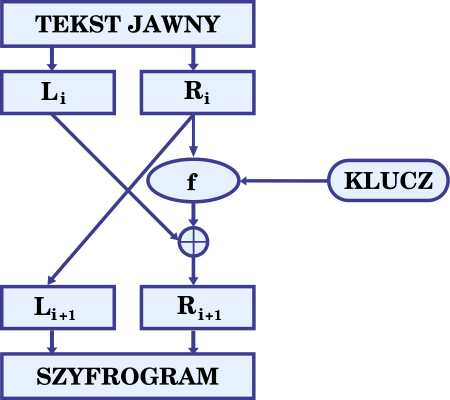
\includegraphics[width=0.3\textwidth]{rozdziały/images/BSK/siec-feistela.png}
\end{figure}

\begin{figure}[H]
    \centering
    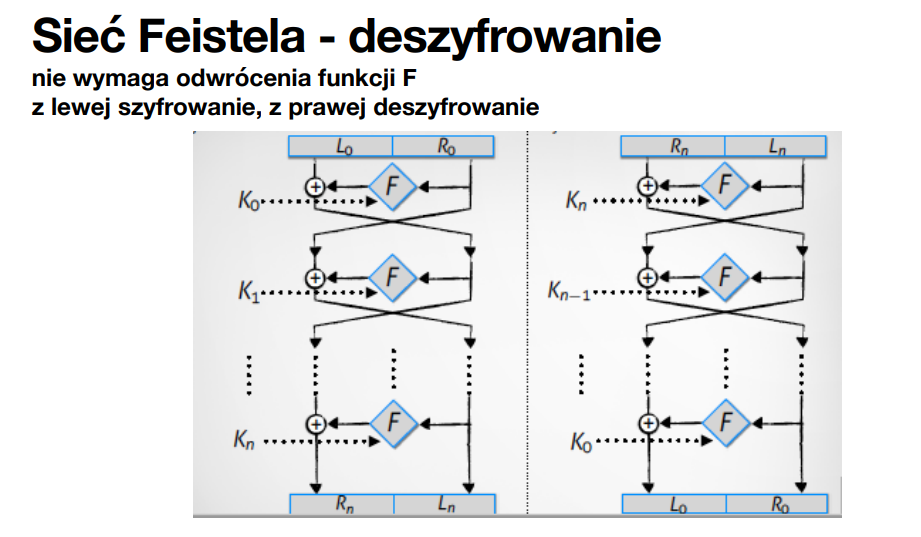
\includegraphics[width=0.75\textwidth]{rozdziały/images/BSK/siec-feistela-dec.png}
\end{figure}

DES jest przestarzały, obecnie używa się \textbf{3DES} (szyfrowanie 3 razy z różnymi kluczami) albo \textbf{AES}

Szyfrowanie tych samych bloków jeden po drugim może dać dodatkową informację więc stosuje się sztuczki np. \textbf{CTR (counter)}

\begin{figure}[H]
    \centering
    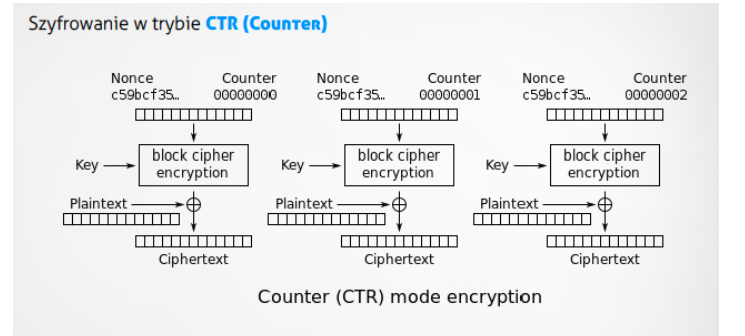
\includegraphics[width=0.75\textwidth]{rozdziały/images/BSK/ctr.png}
\end{figure}

\subsection{Haszowanie, MAC}

\begin{figure}[H]
    \centering
    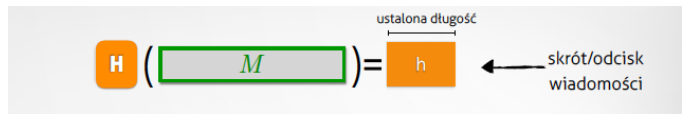
\includegraphics[width=0.75\textwidth]{rozdziały/images/BSK/haszowanie.png}
\end{figure}

Funkcja haszująca (\textbf{funkcja skrótu}) jest:
\begin{itemize}
    \item deterministyczna

    \item łatwo obliczalna

    \item trudno odwracalna

    \item odporna na kolizje
\end{itemize}

Przykłady funkcji hashujących:

\begin{itemize}
    \item SHA-1 - 160 bitów

    \item SHA-2 - 224, 256, 384, 512 bitów

    \item SHA-3 - 224, 256, 384, 512 bitów

    
\end{itemize}

Z hashowania korzysta się w generowaniu \textbf{MACa} czyli krótkiej informacji umożliwiającej weryfikację autentyczności

t = MAC(m, K)

MAC pełni rolę podpisu cyfrowego - nie służy do utajniania wiadomości. Naiwne MACi są podatne na ataki więc w protokołach TLS/SSL i IPSec stosuje się \textbf{HMAC}.


\begin{figure}[H]
    \centering
    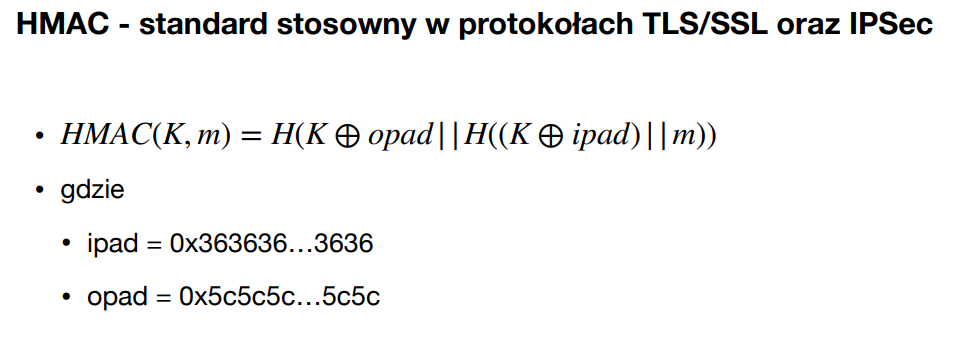
\includegraphics[width=0.75\textwidth]{rozdziały/images/BSK/hmac.png}
\end{figure}

\begin{problems}

    \prob Od kryptograficznej funkcji skrótu $f$ wymagamy, aby dla danego $x$ trudne obliczeniowo było znalezienie takiego $y\neq x$, że
    \answers{$f(f(y))=x$}{$f(x)=f(y)$}{$f(y)=x$}
    
\end{problems}    


\section{Protokół Diffiego-Hellmana, problem logarytmu dyskretnego}

Jak dotychczas zakładaliśmy, że obie strony mają utajniony klucz. Ale jak tego dokonać, żeby było bezpiecznie? Z pomocą przychodzi protokół Diffiego-Hellmana.

Wybieramy grupę cykliczną $G$ z generatorem $g$. Powszechnie stosuje się grupy mnożenia modulo liczba pierwsza i grupy dodawania punktów na krzywej eliptycznej.

\begin{figure}[H]
    \centering
    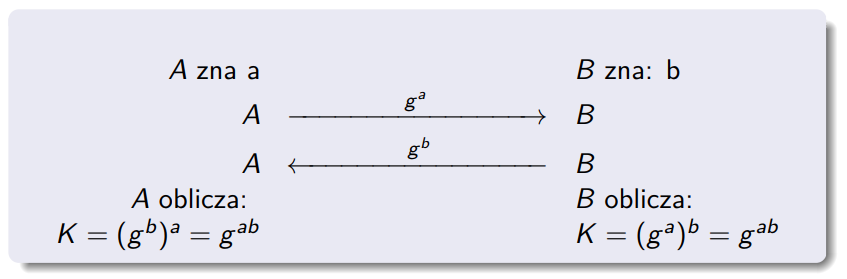
\includegraphics[width=0.75\textwidth]{rozdziały/images/BSK/dh1.png}
\end{figure}

Podsłuchujący zna $g, g^a, g^b$ ale nie pozwala mu to obliczyć K - przy założeniu że wybieramy grupę dla której problem logarytmu dyskretnego (dla danego $g, g^x$ obliczyć $x$) jest obliczeniowo trudny.

Generalnie DH jest fajny ale mamy w nim dosyć mocne założenie że podsłuchujący nie może ingerować w przesyłane wiadomości. Nie zawsze jest to prawda i przykładem jest atak "Man in the middle"

\begin{figure}[H]
    \centering
    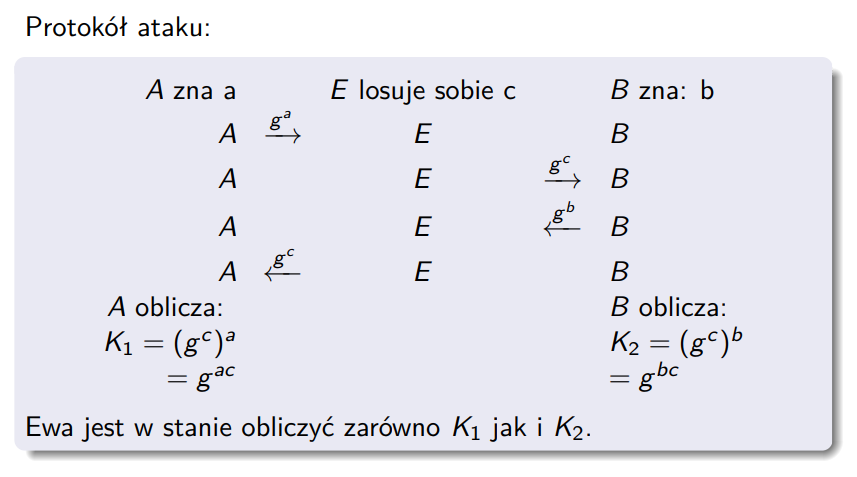
\includegraphics[width=0.75\textwidth]{rozdziały/images/BSK/man-in-the-middle.png}
\end{figure}

W 2015 odkryto że agencje rządowe są w stanie obliczyć logarytm dyskretny liczby 1024-bitowej więc trzeba stosować większe.

Ostatecznie jednak protokół Diffiego-Hellmana nie jest idealny ale nadal się go stosuje w połączeniu z kryptografią klucza publicznego.


\begin{problems}
    
    \prob Po wykonaniu algorytmu Diffiego-Hellmana
    \answers{obie strony znają wspólny sekret}{obie strony poznają dokładnie jeden bit informacji}{obie strony otrzymały komunikat wysłany przez drugą stronę, którego wcześniej nie znały, a~który jest chroniony przed odczytem przez trzecią stronę}
    
\end{problems}    

\section{Kryptografia klucza publicznego}

W takiej kryptografii mamy podział na pary \textbf{PK (public key)} oraz \textbf{SK (secret key)}. Każdy może zaszyfrować swoją wiadomość używając PK ale tylko właściciel SK może ją odszyfrować, dlatego że odwrócenie funkcji szyfrującej opiera się na problemie faktoryzacji.

\subsection{RSA}
RSA to przykład szyfru asymetrycznego

$p, q$ - 2 duże liczby pierwsze

$N = p \cdot q$

$\phi(N) = (p-1)(q-1)$

$e$ - dowolna liczba pierwsza względnie pierwsza z $\phi(N)$

$d = e^{-1} \mod \phi(N)$

$PK = (N, e)$

$SK = (N, d)$

Szyfrogram: C

Szyfrowanie: $C = M^e \mod N$

Deszyfrowanie: $M' = C^d \mod N$

Jak działa to $M' = M$

\subsection{Podpis cyfrowy}
Podpis cyfrowy zapewnia:
\begin{itemize}
    \item autentyczność - możliwość weryfikacji autora

    \item niezaprzeczalność - autor nie może się wyprzeć podpisu

    \item integralność - nie da się dokonać nieautoryzowanej manipulacji podpisanej wiadomości
\end{itemize}

Podpis: $\sigma$ = Sig(SK,M)

Ver(PK, $\sigma$, M) $\in$ {0,1}


Bardzo trudno stworzyć poprawną parę ($\sigma$, M) bez znania SK
Ver(PK, Sig(SK, M), M) = 1

Zwykłe RSA jest za słabe dla podpisu cyfrowego:
\begin{itemize}
    \item kowalność - znając podpisy $\sigma_1, \sigma_2$ dla $M_1, M_2$ można wygenerować podpis dla $M_1 \cdot M_2$

    \item można generować podpisy dla losowych wiadomości

    \item podatność na ataki powtórzeniowe - raz podpisaną wiadomość (np. o treści TAK/WYRAŻAM ZGODĘ etc) można wielokrotnie wykorzystać
\end{itemize}

W praktyce:
\begin{itemize}
    \item dodaje się hasz - zapobiega kowalności i generowaniu losowych wiadomości. 

    \item wiadomości się ulasawia i dodaje timestampy - zapobiega atakom powtórzeniowym
\end{itemize}

Obecnie najczęściej używa się RSA-PSS.

Istnieje również podpis El-Gamala.

\subsection{Certyfikat kluczy publicznych}
Skąd wiadomo że jakiś klucz publiczny jest legit?
Istnieją 2 modele certyfikacji
\begin{itemize}
    \item infrastruktura klucza publicznego PKI - certyfikaty wydawane przez zaufane urzędy

    \item sieć zaufania np. w PGP - użytkownicy wzajemnie poświadczają
\end{itemize}


\begin{problems}
    \prob W kryptografii z kluczem publicznym klucz
    \answers{publiczny służy do szyfrowania i podpisywania cyfrowego}{prywatny służy do deszyfrowania i weryfikowania podpisu cyfrowego}{prywatny służy do szyfrowania, a publiczny do deszyfrowania}
    
    
    \prob Współczesne rekomendacje dla kluczy publicznych używanych w szyfrowaniu RSA określają, że dla zapewnienia dostatecznie bezpiecznej poufnej komunikacji wystarczająca jest długość klucza równa
    \answers{2048 bitów}{1024 bitów}{256 bitów}

    
    \prob Do zabezpieczenia komunikacji od ataku powtórzeniowego stosuje się technikę
    \answers{dodawania numeru kolejnego pakietu do każdego komunikatu}{dodawania timestampów do każdego komunikatu}{stosowania kryptograficznej funkcji haszującej 2 razy}
 
 \end{problems}



\section{Zastosowania kryptografii klasycznej}

Jednym z zastosowań kryptografii klasycznej są wykorzystywane aktualnie sposoby na bezpieczną komunikację w Internecie.

\textbf{Kerberos} - protokół uwierzytelniania z wykorzystaniem KDC (centrum dystrybucji kluczy). Szyfrowanie odbywa się przy użyciu kryptografii symetrycznej. Protokół polega na tym, że każdy użytkownik ma tajny klucz, znany KDC. Gdy użytkownik A chce się skomunikować z B, to zgłasza się do KDC z informacją o planowanej komunikacji. Następnie KDC wysyła do A nowo wylosowany klucz $K_{AB}$ oraz komunikat $C=Enc_{K_B}\{K_{AB}, A\}$ ($K_B$ to tajny klucz B oraz wszystkie wiadomości są zaszyfrowane tajnym kluczem użytkownika A). A wysyła do B komunikat C, dzięki czemu A i B mogą się bezpiecznie komunikować za pomocą klucza $K_{AB}$.

Wzbogacenie standardowego Internetu o szyfrowanie odbywa się poprzez zmianę protokołu komunikacji w różnych warstwach sieciowych. Szyfrowanie nie jest ustalone z góry, przed komunikacją następuje faza negocjacji, w której wybierana jest metoda szyfrowania (tzw. IKE - Internet Key Exchange). Wyróżnia się dwa typy rozszerzonego protokołu:
\begin{itemize}
    \item \textbf{IPsec} - na poziomie sieci, obowiązkowy w IPv6, dodaje szyfrowanie do wysyłanych pakietów (nagłówek IP oraz nagłówek AH/ESP z danymi wykorzystywanymi do uwierzytelniania są jawne, pozostałe dane są zaszyfrowane)
    \item \textbf{TLS} (Transport Layer Security) - podobnie jak IPsec, ale na poziomie sesji. Może zapobiegać atakom man-in-the-middle.
\end{itemize}

\textbf{VPN} (Wirtualna Sieć Prywatna) - utworzenie bezpiecznej sieci wewnątrz niezabezpieczonego Internetu, technicznie realizowane za pomocą IPsec lub TLS.

\textbf{TOR} (The Onion Router) - celem tego systemu jest stworzenie rozwiązania, które utajnia nie tylko treść, ale również sam fakt komunikacji między stronami.

\section{Ataki i obrona}

\subsection{Ataki na aplikacje WWW}
Ataki na aplikacje WWW:
\begin{itemize}
    \item \textbf{atak XSS} (skrośny atak skryptowy) - dotyczy serwisów, które umożliwiają jednemu klientowi uruchamianie skryptów stworzonych przez drugiego klienta,
    \item \textbf{atak XSRF, CSRF} (skrośne fałszowanie żądania) - użytkownik zalogowany do pewnego serwisu uruchamia spreparowany odnośnik (może być uruchomiony gdzieś indziej, np. w innej zakładce), który powoduje wykonanie niechcianej akcji w tym serwisie,
    \item \textbf{wstrzykiwanie kodu SQL}
    \begin{example}
    Rozważamy serwer, który wykonuje zapytanie SQL podstawiając pod zmienne \$login i \$password dane wprowadzone przez użytkownika i akceptując użytkownika, jeśli zapytanie zwróci niezerową liczbę:
    \begin{verbatim}
    SELECT count(*) FROM client WHERE name='$login' and pwd='$password';
    \end{verbatim}
    Możliwy atak: jako login oraz password wpisujemy: d’ or ’1’=’1. Wtedy nasze zapytanie będzie miało postać:
    \begin{verbatim}
    SELECT count(*) FROM client WHERE name='d’ or ’1’=’1' and pwd='d’ or ’1’=’1';
    \end{verbatim}
    Zapytanie to (dla niepustej bazy) nigdy nie zwróci 0, zatem użytkownik zostanie zawsze wpuszczony.
    \end{example}
\end{itemize}

\subsection{Inne ataki}
\textbf{Wirus/robak} to program, który się samoreplikuje. Robak komunikuje się i przyjmuje polecenia od centrali przez sieć, natomiast wirus raz wypuszczony działa samodzielnie.

\textbf{Atak DDoS} (Distributed Denial od Service) - świadome zmasowane zwiększenie ruchu sieciowego (w celu spowolnienia lub czasowego wyłączenia usługi). Jedną z popularnych technik ataku jest wysyłanie dużej ilości małych pakietów do botnetu (duża grupa zainfekowanych komputerów), który z kolei wysyła większe pakiety do atakowanych serwerów. Zaatakowane serwery przestają odpowiadać lub ich łącza internetowe osiągają limit przepustowości.

\textbf{Reverse engineering} - próba analizy kodu binarnego w celu znalezienia w nim luki czy zhardkodowanych danych.

\textbf{Atak buffer overflow} - idea polega na tym, że wprowadzamy jakoś do pamięci atakowanego programu złośliwy kod, tzw. shell code (np. poprzez podanie go jako argument wejściowy). Następnie zmieniamy poprawne działanie atakowanego programu zmieniając mechanizmy sterowania wykonaniem programu (np. poprzez nadpisanie w pamięci adresu powrotu z wykonywanej funkcji). To właśnie da się osiągnąć dzięki między innymi przepełnieniu buforu (buffer overflow), który występuje wtedy, gdy zapisujemy do wyznaczonego buforu większej ilości danych, niż była zarezerwowana. Dzięki temu możemy stworzyć na tyle dużo obiektów w ramach sterty, aby zahaczyć o stos i odpowiednio nadpisać adres powrotu do wykonywanej funkcji.

Techniki obrony przed atakiem buffer overflow:
\begin{itemize}
    \item \textbf{kanarek} - unikalna wartość umieszczana na stosie między zmiennymi a adresem powrotu, sprawdzana przed wykonaniem powrotu,
    \item DEP (data execution prevention) - OS nie pozwala na wykonanie kodu umieszczonego dynamicznie na stercie (choć musi zrobić wyjątek dla bibliotek ładowanych dynamicznie).
\end{itemize}

\textbf{ROP} (return oriented programming) - atak polegający na nie korzystaniu z shell code, tylko skakaniu do kodu atakowanego programu w odpowiednio dobrane miejsca, z których atakujący skleja złośliwą funkcjonalność.

\textbf{Buffer overread} - atakujący, manipulując wskaźnikami, dostaje możliwość odczytu pamięci, której nie powinien widzieć.

\begin{problems}
    \prob Atak DDoS polegający na wysyłaniu wielu nieukończonych fragmentów pakietów IP działa, ponieważ
    \answers{na komputerze docelowym wyczerpany zostaje limit zasobów na obsługę pakietów}{na oprogramowaniu pewnego rutera pośredniczącego wyczerpany zostaje limit zasobów na obsługę pakietów}{przekroczony zostaje MTU}

    \prob Aby utrudnić dokonywanie ataków poprzez przepełnienie stosu (ang. \textit{stack overflow}), można
    \answers
    {przekazywać argumenty w rejestrach zamiast na stosie}
    {alokować wszystkie bufory na stercie zamiast na stosie}
    {użyć architektury RISC, w której występuje specjalny rejestr LR (ang. \textit{link register}), który zawiera adres powrotu do funkcji wołającej}
\end{problems}

\begin{solutions}
    % Grześ
    \sol Od kryptograficznej funkcji skrótu $f$ wymagamy, aby dla danego $x$ trudne obliczeniowo było znalezienie takiego $y\neq x$, że
    \answerss{$f(f(y))=x$}{$f(x)=f(y)$}{$f(y)=x$}{TAK}{TAK}{TAK}
    \textbf{A.} Chcemy, żeby obliczeniowo trudne było znalezienie jakiejkolwiek własności $f$, której nie powinniśmy znać. W tym przypadku potrafilibyśmy odszyfrowywać wiadomości zaszyfrowane dwukrotnie, czego raczej nie chcemy.

    \textbf{B.} W tej sytuacji, łatwo by było znaleźć inną wiadomość, która jest taka sama jak oryginalna po zaszyfrowaniu. Można by wtedy przechwycić oryginalną wiadomość, a do odbiorcy wysłać jakiś śmieć.

    \textbf{C.} Tutaj to już w ogóle tragedia, bo moglibyśmy czytać zaszyfrowane wiadomości.

    % Grześ
    \sol Po wykonaniu algorytmu Diffiego-Hellmana
    \answerss{obie strony znają wspólny sekret}{obie strony poznają dokładnie jeden bit informacji}{obie strony otrzymały komunikat wysłany przez drugą stronę, którego wcześniej nie znały, a~który jest chroniony przed odczytem przez trzecią stronę}{TAK}{NIE}{NIE}
    \textbf{A.} Tak, obydwaj znają $g^{ab}$, dzięki czemu mogą się komunikować.

    \textbf{B.} Nie bardzo.

    \textbf{C.} Zdanie jest obiecujące, ale ostatnia część ,,który jest chroniony przed odczytem przez trzecią stronę" jest nieprawdą.

    % Patryk
    \sol W kryptografii z kluczem publicznym klucz
    \answerss{publiczny służy do szyfrowania i podpisywania cyfrowego}{prywatny służy do deszyfrowania i weryfikowania podpisu cyfrowego}{prywatny służy do szyfrowania, a publiczny do deszyfrowania}{NIE}{NIE}{NIE}
    \textbf{A.} Do podpisywania cyfrowego służy klucz prywatny.

    \textbf{B.} Do weryfikowania podpisu służy klucz publiczny.

    \textbf{C.} Na odwrót.

    % Grześ
    \sol Współczesne rekomendacje dla kluczy publicznych używanych w szyfrowaniu RSA określają, że dla zapewnienia dostatecznie bezpiecznej poufnej komunikacji wystarczająca jest długość klucza równa
    \answerss{2048 bitów}{1024 bitów}{256 bitów}{TAK}{NIE}{NIE}
    Jak wiemy, agencje rządowe potrafią obliczyć logarytm dyskretny liczby 1024-bitowej w skończonym czasie, ale 2048 bitów jest już bezpieczne.

    % Julia
    \sol Do zabezpieczenia komunikacji od ataku powtórzeniowego stosuje się technikę
    \answerss{dodawania numeru kolejnego pakietu do każdego komunikatu}{dodawania timestampów do każdego komunikatu}{stosowania kryptograficznej funkcji haszującej 2 razy}{TAK}{TAK}{NIE}

    \textbf{A.} Numery kolejnych pakietów mogą działać jak swego rodzaju timestampy, o których mowa w podpunkcie poniżej \\
    \textbf{B.} Dodanie timestampów pozwala na uniknięcie ataku powtórzeniowego, ze względu na to, że powtórnie użyty komunikat będzie miał zapisany inny timestamp niż czas ponownego użycia \\
    \textbf{C.} Podwójne zastosowanie funkcji haszującej nie pozwoli na uniknięcie ponownego wykorzystania komunikatu

    \sol Atak DDoS polegający na wysyłaniu wielu nieukończonych fragmentów pakietów IP działa, ponieważ
    \answerss{na komputerze docelowym wyczerpany zostaje limit zasobów na obsługę pakietów}{na oprogramowaniu pewnego rutera pośredniczącego wyczerpany zostaje limit zasobów na obsługę pakietów}{przekroczony zostaje MTU}{NIE}{TAK}{NIE}
    
    \sol Aby utrudnić dokonywanie ataków poprzez przepełnienie stosu (ang. \textit{stack overflow}), można
    \answerss
    {przekazywać argumenty w rejestrach zamiast na stosie}
    {alokować wszystkie bufory na stercie zamiast na stosie}
    {użyć architektury RISC, w której występuje specjalny rejestr LR (ang. \textit{link register}), który zawiera adres powrotu do funkcji wołającej}
    {TAK?}{TAK?}{NIE?}

    % \sol Atak przez odtworzenie ruchu (ang. \textit{replay}) polega na tym, że
    % \answerss{atakujący w celu uzyskania zamierzonego efektu odsyła atakowanemu literalną kopię komunikatu, jaki właśnie od niego uzyskał}{atakujący pozyskuje fragment interakcji między uprawnionymi użytkownikami, a następnie w~innym kontekście używa go do uzyskania zamierzonego celu}{atakujący dokonuje pełnego zrzutu ruchu w sieci lokalnej w jakimś odcinku czasu, a następnie wysyła do sieci ruch, za którego pomocą usiłuje doprowadzić do sytuacji, w której ruch będzie wyglądał dokładnie tak, jak w uzyskanym zrzucie}{NIE}{TAK}{NIE}
\end{solutions}
